\section{King Rao 1992}
\label{KR92Secton}

V. King and S. Rao published in \cite{King1992} an algorithm which runs in time $O(nm+n^{2+\varepsilon})$ for any $\varepsilon>0$.
The main part of the algorithm is based on a Push Relabel algorithm by J. Cheriyan, T. Hagerup and K. Mehlhorn \cite{Cheriyan1990}. 
The contributions done by \cite{King1992} are primarily modifications to a subroutine called the game. 
The purpose of the game is to select current edges, which determines which edge to push on when pushing excess from a node.

The game subroutine is described as a game played between the algorithm and an adversary. 
Cheriyan {\it et al.} \cite{Cheriyan1990} showed that their algorithm runs in $O(nm + n^{2/3}m^{1/2}+P(n^2, nm)+C(n^2, nm))$, 
where the function $P : \mathbb{N}\times\mathbb{N}\to\mathbb{N}$ represents the number of points scored by the adversary in the game, 
and $C : \mathbb{N}\times\mathbb{N}\to\mathbb{N}$ represents the cost of implementing the algorithm's game strategy. 
The algorithm by Goldberg and Tarjan \cite{Goldberg1988} chooses the edges in any order. 
By selecting a specific order that aims to more effectively spread the flow in the graph, the worst case time can be reduced.
 
In Section~\ref{KRGameSection}, we will describe the general game, without relating it to the algorithm. 
We will then argue for the bounds on $P$ and $C$ in Section~\ref{KRGameAnalysisSection}.
Section~\ref{KRAlgorithmSection} will contain the main algorithm, and its relation to the game,
and in Section~\ref{KRAlgorithmAnalysisSection}, we will show how the algorithm achieves the runtime of $O(nm+n^{2+\varepsilon})$.
Finally, the algorithm turned out to have some issues in practice, especially related to memory consumption. 
In Section~\ref{KRModificationsSection} we will describe the modifications we have done to make the algorithm more usable in practice, including reducing the memory requirement while staying within the same theoretical bound.


\subsection{The Game}
\label{KRGameSection}

The game is played between the player and the adversary on a bipartite graph $G_g=(U_g, V_g, E_g)$.
We will use $N$ to signify the number of nodes, and $M$ to signify the number of edges, such that $N=|U_g|=|V_g|$, $M=|E_g|$.
This is not the same graph as the graph $G$ we run max flow on, but we will describe how to construct $G_g$ from $G$ in Section~\ref{KRAlgorithmSection}.
For every node $u\in U_g$, the player must at all times have chosen a single edge incident to $u$ to be the designated edge, unless no edges are incident to $u$.
Certain moves done by the player or the adversary on these designated edges might award points to the adversary.

The goal for the player is to minimize the amount of points gained by the adversary.
We use $P(N, M)$ to represent the points scored by the adversary, and $C(N, M)$ to represent the cost of implementing the player's strategy.
The moves the adversary can do are:
\begin{description}
  \item[Edge kill] \hfill \\
  The adversary can kill any edge $(u, v)$, permanently removing it from the game. He scores no points for this move.
  
  \item[Node kill] \hfill \\
  The adversary can kill any node $v \in V_g$, permanently removing it and all incident edges from the game. He scores a point for every edge removed that was a designated edge.
\end{description}
The player can respond with any sequence of the following moves:
\begin{description}
  \item[Edge designation] \hfill \\
  The player must designate an edge for each node $u\in U_g$ that does not currently have a designated edge,
  unless no edges are incident to $u$.
  
  \item[Edge redesignation] \hfill \\
  The player can change the designated edge of a node $u\in U_g$ that already have a designated edge, but he awards a point to the adversary for this move.
\end{description}

\begin{figure}[!ht]
\centering
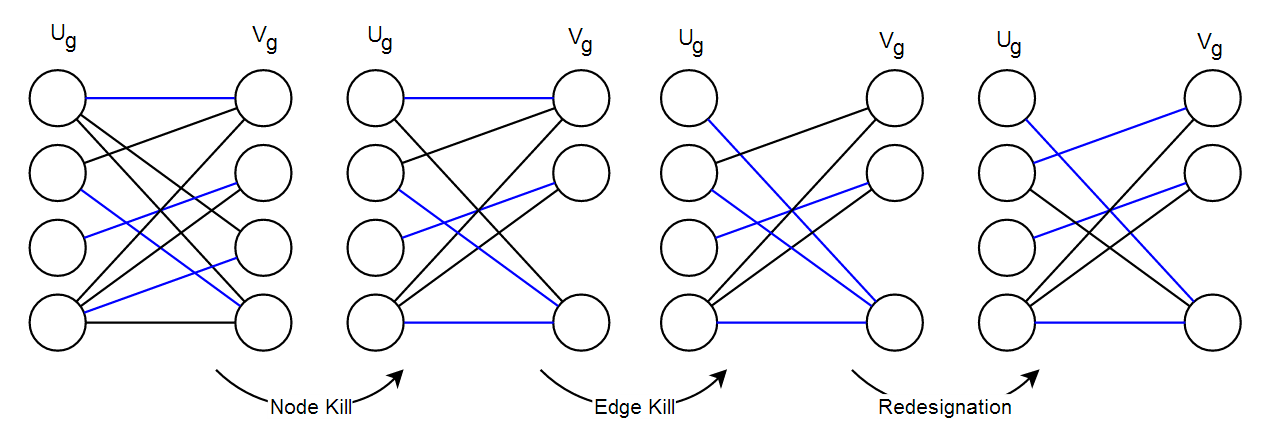
\includegraphics[width=120mm]{KRGameExample.png}
\caption{An example of moves in the game. The adversary gains two points from these moves.}
\label{akExample}
\end{figure}

\begin{algorithm}
\caption{The game of \cite{King1992}}\label{King1992Game}
\begin{algorithmic}[1]
\Procedure{AdversaryNodeKill}{$v$}
	\State Perform {\sc AdversaryEdgeKill} on all edges incident to $v \in V_g$
\EndProcedure
\Procedure{AdversaryEdgeKill}{$u$, $v$}
	\State Remove $(u, v)$ from the game
	\If {$(u, v)$ was the designated edge of $u$}
		\If {$u \in U_g'$}
			\State {\sc UpdateRatioLevel}($v$)
		\EndIf
		\State {\sc DesignateEdge}($u$)
	\EndIf
\EndProcedure
\Procedure{DesignateEdge}{$u$}
	\If{$degree(u) \leq l$}
		\State Designate any edge incident to $u \in U_g$
	\Else
		\State Designate edge $(u, v)$ such that $erl(v)$ is minimal over all edges incident to $u$
		\State {\sc UpdateRatioLevel}($v$)
	\EndIf
\EndProcedure
\Procedure{UpdateRatioLevel}{$v$}
	\If {$erl(v) \not\in [rl(v), rl(v)+1]$}
		\State $erl(v) \gets rl(v)$
		\If {$erl(v) = t$}
			\State {\sc Reset}()
		\EndIf
	\EndIf
\EndProcedure
\Procedure{Reset}{}
	\State $k \gets t$
	\While {$|U_{k-2}|\geq(r_{k-1}l)|U_k|/4$}
		\State $k \gets k - 2$
	\EndWhile
	\State Set $erl(v) \gets rl(v)$ for all $v \in V_{k-2}$
	\State Undesignate the designated edge for all $u \in U_k$
	\State Set $erl(v)=rl(v)=0$ for all $v \in V_k$
	\State Designate an edge for all $u \in U_k$
\EndProcedure

\end{algorithmic}
\end{algorithm}
The game starts with the player designating edges. Then it progresses by repeatedly having the adversary do a move, followed by zero or more moves by the player.

The strategy we will use for the player takes three parameters; $l$,~$t$~and~$r_0$. 
For nodes $u$ with fewer than $l$ edges, we will simply designate any edge.
We thus define $U_g'=\{u \in U_g \mid \mathrm{degree}(u) > l\}$ as the subset of $U_g$ where we use the advanced strategy.

We define the ratio $r(v)$ of a node $v \in V_g$ as $r(v)=\frac{\mathrm{degree_{designated}}(v)}{\mathrm{degree_{initial}}(v)}$, 
where $\mathrm{degree_{designated}}(v)$ is the number of designated edges to $v$ from nodes in $U'$, and $\mathrm{degree_{initial}}(v)$ is the degree of $v$ before any edges was removed.
The idea for the player's strategy is, when designating an edge $u \in U_g$, to look at all $v \in V_g$ incident to $u$, and designate the edge to the node $v$ with the lowest $r(v)$.
This way, the adversary won't score that many points when he performs a node kill. 
It will be too expensive to maintain a sorted list of ratios for every $u$ though, so we partition them into ratio levels $rl(v)$.

We use $t$ to represent the highest ratio level allowed, and $r_0$ as a seed for when a node changes ratio level.
We define
\begin{align*}
r_i&=2^ir_0 \forall i \in \{1, ..., t\}\\
rl(v)&=\left\{
\begin{aligned}
0 &\text{ if }r(v)<r_0\\
i &\text{ if }r_i \leq r(v)< r_{i+1}\\
t &\text{ if }r_t \leq r(v)
\end{aligned}
\right.
\end{align*} 

Instead of keeping track of the ratio level of all nodes in $V_g$, we keep track of the estimated ratio level $erl(v)$, which might not represent the exact ratio level.
When the ratio level of a node increases, we update the estimated ratio level to reflect the change, but when it decreases, 
we don't update the estimated ratio level until the ratio level has decreased twice. 
The reason behind this is that we want to avoid doing a lot of work if a ratio level oscillates between two levels.

The goal of the strategy is to make sure that $erl(v)$ is low when $v$ is killed. We make an invariant that says that $erl(v) < t$ for all $v \in V_g$ at the end of the player's turn. 
This means that no node $v$ can be killed while having $erl(v)\geq t$.\\

The strategy for the player is as follows. 
When the game starts, the player must designate an edge for each node in $U_g$. When designating an edge for a node $u$, we designate any edge if $degree(u)<l$, 
and otherwise an edge $(u, v)$ such that $erl(v)$ is minimal over all incident edges. If this causes the ratio level of $v$ to increase, we must update its estimated ratio level.

When the adversary kills a designated edge $(u, v)$, either through a node kill or an edge kill, the player designates a new edge for $u$.
If as a result of an edge designation, the estimated ratio level of a node $v$ becomes equal to $t$, the player performs a reset operation.
The reset operation performs a number of edge redesignations to reduce the estimated ratio levels of all nodes above a certain level. 

When doing a reset, we place the nodes into sets based on their ratio level.
We define $V_i$ to be all nodes $v\in V_g$ with $rl(v) \geq i$, and $U_i$ to be all nodes $u \in U_g'$ whose designated edge goes to a node in $V_i$.
\begin{align*}
V_i&=\left\{v\in V_g\mid rl(v) \geq i\right\}\\
U_i&=\left\{u \in U_g'\mid  \mathrm{designatedEdge_{target}}(u) \in V_i\right\}
\end{align*}
Let $k>3$ be the last level that satisfies $|U_{k-2}|<(r_{k-1}l)|U_k|/4$.
The reset operation first updates the $erl$ of all $v$ with $rl(v)=k-2$, so $erl(v)$ gets the current value of $rl(v)$. 
It then undesignates all designated edges from nodes in $U_k$, and updates $rl$ and $erl$ for all nodes in $V_k$ to 0.
Finally, it redesignates edges for nodes in $U_k$.

\subsection{Analysis of The Game}
\label{KRGameAnalysisSection}


In this section we will argue for the points gained by the adversary $P(N, M)$, and the cost of implementing the player's strategy $C(N, M)$.\\

First, we will bound the value of $P(N, M)$.
The adversary gains a point when he kills a designated edge while killing a node, and when the player redesignates an edge.

When the degree of a node $u$ falls below $l$, we will award $l$ points to the adversary for the remaining edges.
This is the maximum amount of points he could possibly score for $u$ in the remainder of the game, since we will not redesignate any edges for nodes $u \not\in U_g'$. 
Every node in $U_g$ only drops below $l$ once, so the total number of points that can be gained this way is $l N$.

When the adversary performs a node kill on $v$, he gains $\mathrm{degree_{designated}}(v)$ points. 
But due to the reset procedure, a node can not be in ratio level $t$ or above when it is removed. 
We then get the inequalities
\begin{align*}
r(v) &\leq r_{t-1}\\
\frac{\mathrm{degree_{designated}}(v)}{\mathrm{degree_{initial}}(v)} &\leq r_{t-1}\\ 
\mathrm{degree_{designated}}(v) &\leq r_{t-1} \mathrm{degree_{initial}}(v)\\ 
\sum\limits_{v\in V_g}{\mathrm{degree_{designated}}(v)} &\leq r_{t-1}\sum\limits_{v\in V_g}{\mathrm{degree_{initial}}(v)}\\ 
points &\leq r_{t-1} M
\end{align*}
The number of points the adversary can gain this way is thus at most $r_{t-1}M$, because a node only can be killed once.

The last source of points are the redesignations done by the player. All of these are done in the reset procedure of the strategy.
We will show that when a reset occurs on level $k$, there have been many edge kills since the last reset on level $k$. 
We can then assign the cost of the redesignations to these edge kills.
When we say that a reset occurs on level $k$, we mean that it redesignateded edges for all $u \in U_k$.
In the following sections we will argue about what happened previous to a reset on level $k$. Specifically, what has happened since the previous reset on level $k$, or since the start of the algorithm.
\begin{lemma}
\label{KRGame1}
When a reset occurs on level $k$, there has been at least $r_{k-1}l|U_k|/2$ designated edges to nodes in $V_{k-1}$ since the previous reset at or below level $k$, or the start of the algorithm if no such reset has occurred.
\end{lemma}
\begin{proof}
Let $v \in V_k$, and let $U_k(v)=\left\{u\in U_k \mid  designatedEdge_{target}(u) = v\right\}$. 
The size of $U_k(v)$ is $\mathrm{degree_{designated}}(v)$, due to the definition of $U_k$.
At the time that $(u, v)$ was designated, $erl(v)$ must have been the smallest $erl$ amongst all neighbours of $u$.
Since $v \in V_k$, $erl(v)$ must have been at least $k-1$, and since it was the smallest $erl$, the $erl$ of all neighbours of $u$ must also have been at least $k-1$.
At some point since the last reset at or below level $k$ or since the start of the algorithm, $rl(v)$ must have been less than $k$.
Further more, the $erl$ of all neighbours to $u$ must have been below~$k$, 
because all nodes start out with $rl(v)=0$, and the reset procedure resets the ratio levels of nodes with $rl(v) \geq k$ to $0$. 

For $rl(v)$ to increase from $0$ to $k$, at least $|U_k(v)|/2$ edge designations must have been done to $v$.
Since all nodes in $u \in U_g'$ have $degree(u)>l$, there must have been $l|U_k(v)|/2$ edges incident to nodes in $V_{k-1}$ since the previous reset at level $k$ or lower.
These edges are the edges incident to $u$ that are not designated.
If we sum this up over all $v \in V_k$, we get $l|U_k|/2$ edges incident to nodes in $V_{k-1}$, because all $U_k(v)$ are disjoint.

We can then calculate how many designated edges there must be for a node $w \in V_{k-1}$, and for all nodes in $V_{k-1}$.

\begin{align*}
r_{k-1} &\leq r(w) \\
r_{k-1} &\leq \frac{\mathrm{degree_{designated}}(w)}{\mathrm{degree_{initial}}(w)}\\
\mathrm{degree_{designated}}(w) &\geq r_{k-1}\mathrm{degree_{initial}}(w)\\
\sum\limits_{w\in V_{k-1}}{\mathrm{degree_{designated}}(w)} &\geq r_{k-1}\sum\limits_{w\in V_{k-1}}{\mathrm{degree_{initial}}(w)} \\
\sum\limits_{w\in V_{k-1}}{\mathrm{degree_{designated}}(w)} &\geq r_{k-1}l|U_k|/2
\end{align*}
For each individual $w$, this only holds at the time the edge $(u, v)$ was designated, 
so the sum says that there has been $r_{k-1}l|U_k|/2$ designated edges to nodes in $V_{k-1}$ since the previous reset at or below level $k$, or the start of the algorithm.
$\square$
\end{proof}
\begin{lemma}
\label{KRGame2}
At any point in the algorithm, at every level $k \geq 3$, at least one of the following two statements hold:
\begin{enumerate}
  \item $|U_{k-2}|\geq r_{k-1}l|U_k|/4$.
  \item There was at least $r_{k-1}l|U_k|/8$ edge kills at level $k-2$ or higher, since the previous time a reset occured at or below level $k$.
\end{enumerate}
\end{lemma}
\begin{proof}
To prove this lemma, we will assume that condition 1 does not hold, and show that condition 2 must hold.
Lemma~\ref{KRGame1} gives us that there has been $r_{k-1}l|U_k|/2$ edge designations to nodes in $V_{k-1}$ since last reset at level $k$ or below, but if $|U_{k-2}|< r_{k-1}l|U_k|/4$,
at least $r_{k-1}l|U_k|/4$ designated edges were removed by the adversary from nodes that are or had been in $V_{k-1}$.
A node that drops from level $k-1$ to below $k-2$ must lose at least half its designated edges at level $k-2$, which implies that at least $r_{k-1}l|U_k|/8$ designated edges was removed when they were incident to nodes $v$ with $rl(v) \geq k-2$.
That means that if condition 1 does not hold, then condition two must hold.
$\square$
\end{proof}
When a reset occurs at level $k$, we ensure that condition 1 from Lemma~\ref{KRGame2} does not hold.
The reset performs $|U_k|$ redesignations, and there have been at least $r_{k-1}l|U_k|/8$ edge kills at level $k-2$ or above since the previous reset at level $k$ or below.
We will let $\mathrm{\#edgeKills}_k$ represent the number of edge kills since last reset on level $k$, and $\mathrm{\#redesignations}_k$ to represent the number of redesignations during the specific reset operation.
This gives us the equation 
\begin{align*}
\mathrm{\#edgeKills}_k &\geq \frac{r_{k-1}l|U_k|}{8} \\
\mathrm{\#edgeKills}_k &\geq \frac{r_0l\mathrm{\#redesignations}_k}{8} \\
\mathrm{\#redesignations}_k&\leq\frac{8\mathrm{\#edgeKills}_k}{r_0l} \\
\sum\limits_{\text{All Resets}}{\mathrm{\#redesignations}_k} &\leq \sum\limits_{\text{All Resets}}{\frac{8\mathrm{\#edgeKills}_k}{r_0l}} \\
\mathrm{\#redesignations} &\leq \frac{8\mathrm{\#edgeKills}}{r_0l}
\end{align*}
So, the total points scored by the adversary is
\begin{align*}
P(N, M) \leq N\cdot l + r_{t-1}M + \frac{8\mathrm{\#edgeKills}}{r_0l}
\end{align*}
To make this more interesting, we can assign some values to the parameters $r_0$, $l$ and $t$.
\begin{align*}
r_0 &= \frac{N^\varepsilon}{\sqrt{M/N}}\\
l &= N^\varepsilon \sqrt{M/N}\\ 
t &= O(1/\varepsilon)
\end{align*}
When we insert this into our bound on $P(N, M)$ we get
\begin{align*}
P(N, M) &\leq N\cdot N^\varepsilon \sqrt{M/N} + 2^{\frac{1}{\varepsilon} - 1} \frac{N^\varepsilon}{\sqrt{M/N}}M + \frac{8\mathrm{\#edgeKills}}{N^{2\varepsilon}}\\
&=N^{0.5+\varepsilon}M^{0.5}+2^{\frac{1}{\varepsilon} - 1}N^{0.5+\varepsilon}M^{0.5}+\frac{8\mathrm{\#edgeKills}}{N^{2\varepsilon}}\\
&=O\left(N^{0.5+\varepsilon}M^{0.5} + \frac{\mathrm{\#edgeKills}}{N^{\varepsilon}}\right)
\end{align*}

Next, we will bound the value of $C(N, M)$, which was the cost of implementing the player's strategy.
The algorithm will have to do the following things:

It will need to be able to find the neighbour with minimum $erl$ when designating an edge.
To do this easily, we keep an array of size $t$ of linked lists for each node $u \in U_g'$. 
An edge will be placed in the $i^\mathrm{th}$ linked list, if the corresponding node $v$ has $erl(v)=i$.
This means that we can designate an edge in $O(t)$ time, by enumerating the linked lists from $0$ to $t$, and pick any edge from the first non-empty linked list.
For nodes $u \in U_g \setminus U_g'$, we just keep a single linked list of edges.
There are $P(N, M)+N$ designations in total, so the designations require $O(tP(N, M)+tN)$ time.

An edge can be removed from this data structure in constant time by keeping a pointer to the linked list element in the edge object.
The edges are never added back, so this takes $O(M)$ time total.

The data structure will have to be updated when the $erl$ for a node $v$ changes. 
This means enumerating over all the edges incident to $v$, and moving each edge it into another linked list.
The $erl$ of a node is updated when $rl$ increases by one or decreases by two, and during the reset operation.
If we only consider the first two cases, at least $r_0 \, \mathrm{degree_{initial}}(v)$ edge kills or designations must have occured before the $erl$ of a node changes.
The cost of updating the data structure is $degree(v)$, 
so the cost for all updates to $v$ is at most
\begin{align*}
cost(v) &\leq degree(v)\frac{\mathrm{\#edgeKills}(v) + \mathrm{\#edgeDesignations}(v)}{r_0 \mathrm{degree_{initial}}(v)}\\
 &\leq \frac{\mathrm{\#edgeKills}(v) + \mathrm{\#edgeDesignations}(v)}{r_0}\\
\sum\limits_{v\in V_g}{cost(v)} &\leq \sum\limits_{v\in V_g}{\frac{\mathrm{\#edgeKills}(v) + \mathrm{\#edgeDesignations}(v)}{r_0}}\\
 &\leq \frac{\mathrm{\#edgeKills} + P(N, M) + N}{r_0}
\end{align*}

Finally, we have the updates to $erl$ during the reset operation. The $erl$ is only updated for nodes in or above level $k-2$.
For nodes in $V_{k-2}$, we have
\begin{align*}
r_{k-2} &\leq r(v)\\
r_{k-2} &\leq \frac{\mathrm{degree_{designated}}(v)}{\mathrm{degree_{initial}}(v)}\\
\mathrm{degree_{initial}}(v) &\leq  \frac{\mathrm{degree_{designated}}(v)}{r_{k-2}}\\
\sum\limits_{v\in V_{k-2}}{\mathrm{degree_{initial}}(v)} &\leq  \sum\limits_{v\in V_{k-2}}{\frac{\mathrm{degree_{designated}}(v)}{r_{k-2}}}\\
\sum\limits_{v\in V_{k-2}}{\mathrm{degree_{initial}}(v)} &\leq  \frac{|U_{k-2}|}{r_{k-2}}
\end{align*}
So there are at most $|U_{k-2}|/r_{k-2}$ edges incident to nodes in $V_{k-2}$.
As part of the reset, we ensure that $|U_{k-2}|<r_{k-1}l|U_k|/4$, so we can bound the number of edges further by
\begin{align*}
\sum\limits_{v\in V_{k-2}}{\mathrm{degree_{initial}}(v)} \leq \frac{|U_{k-2}|}{r_{k-2}} < \frac{r_{k-1}l|U_k|}{4r_{k-2}} = \frac{2r_{k-2}l|U_k|}{4r_{k-2}} = \frac{l|U_k|}{2}
\end{align*}
Each reset occurs after at least $r_{k-1}l|U_k|/8$ edge kills, so the cost of updating all the edges are
\begin{align*}
cost &< \frac{l|U_k|}{2} \\
&< \frac{l}{2}\frac{8\mathrm{\#edgeKills}}{r_{k-1}l}  \\
&< \frac{4\mathrm{\#edgeKills}}{r_0} \\
&=O\left( \frac{\mathrm{\#edgeKills}}{r_0} \right)
\end{align*}
This brings the total cost for $C(N, M)$ to
\begin{align*}
C(N, M)&=O\left(tP(N, M)+tN + M + \frac{\mathrm{\#edgeKills} + P(N, M) + N}{r_0}\right)
\end{align*}
We can show that $t < \frac{1}{r_0}$ by
\begin{align*}
r_t &\leq 1\\
2^tr_0 &\leq 1\\
2^t &\leq \frac{1}{r_0}
\end{align*}
By using the fact that $t < 2^t$ for $t \geq 0$, we get $t < \frac{1}{r_0}$.

The final total cost for maintaining the game becomes 
\begin{align*}
C(N, M)=O\left(M + \frac{\mathrm{\#edgeKills} + P(N, M) + N}{r_0}\right)
\end{align*}

\subsection{The Algorithm}
\label{KRAlgorithmSection}


\begin{algorithm}
\caption{\cite{King1992}}\label{King1992Alg}
\begin{algorithmic}[1]
\Function{MaxFlow}{$V, E, s, t$}
	\State Initialize()
	\State $edges \gets \{(u, v)\in E \mid  u \neq s \wedge v \neq s \wedge u < v\}$ 
	\ForAll{$(u, v) \in edges$ ordered by $ucap(u, v)$ decreasing}
		\State Add $(u, v)$ and $(v, u)$ to $F$
		\If{$d(u) > d(v)}$
		\State Saturate$(u, v)$
		\ElsIf{$d(u) < d(v)$}
		\State Saturate$(v, u)$
		\EndIf
		\While{$\exists v \in V\setminus\{s, t\} : e^{*}(v)>0$}
			\If{$CurrentEdge(v) \neq nil$}
				\State TreePush$(v)$
			\Else
				\State Relabel$(v)$
			\EndIf
		\EndWhile
	\EndFor
	\State \textbf{return} $e(t)$
\EndFunction
\Procedure{Initialize}{}
\State Create dynamic forest $F$
\State $d(s) \gets n$
\ForAll{$(s, v) \in E$}
	\State Add $(s, v)$ and $(v, s)$ to $F$
	\State Saturate$(s, v)$
\EndFor
\EndProcedure
\Procedure{TreePush}{$u$}
	\State $(u, v) \gets CurrentEdge(u)$
	\State $link(u, v)$ if not linked
	\If {$\exists$ edge $(x, y)$ on path to root from $u$ in $F : u(x, y) \leq e^*(u)$}
		\State Saturate$(x, y)$
		\State $cut(x, y)$
	\EndIf
	\State send $e^*(u)$ units of flow along path from $u$ to its root in $F$
\EndProcedure
\Procedure{Relabel}{$v$}
	\ForAll {$u\in V : CurrentEdge(u) = (u, v)$}
		\State $cut(u, v)$
	\EndFor
	\State $d(v) \gets d(v)+1$
\EndProcedure
\end{algorithmic}
\end{algorithm}
The algorithm is a version of the push-relabel algorithm, with an additional operation; addEdge. 
It starts out with no edges in the graph, and then adds them one by one as the algorithm progresses.
We define $E^*\subseteq E$ to be the edges that are added to the graph at any point in the algorithm.
The hidden capacity of a node $v$ is defined as $h(v)=\sum\limits_{(v, u)\in E\setminus E^*}{cap(v, u)}$, the sum of capacities on edges going out of $v$ that have not yet been added.
We can then define the \textit{visible excess} to be $e^*(v)=max\left(0, e(v)-h(v)\right)$.
We will use this instead of $e(v)$, to determine when to push or relabel a node.
A push or relabel is only performed if the visible excess of the node is greater than zero, and it is never allowed to push more than the visible excess away from a node.

The initialization is the same as in the algorithm by Goldberg and Tarjan \cite{Goldberg1988}, in that we start with $d(s)=n$ and $\forall v \in V\setminus\{s\}: d(v)=0$. 
We then saturate all edges $(s, v)$ to get some excess into the graph.
Like in the algorithm by Goldberg and Tarjan \cite{Goldberg1988}, a dynamic tree is used to keep track of paths of current edges.

We define the \textit{undirected capacity} of an edge $(u, v)$ to be $ucap(u, v) = cap(u, v) + cap(v, u)$.
The main part of the algorithm adds the edges in order of decreasing $ucap(u, v)$. When $(u, v)$ is added, $(v, u)$ is added as well.

When an edge $(u, v)$ is added, the algorithm checks if $d(u)>d(v)$, and if so, saturates the edge. 
The reason it can do this is that $d(u)>d(v) \Rightarrow d(u)>0$, so $u$ was relabelled at some point.
When $u$ was relabeled, $e^*(u)>0 \Rightarrow h(u)<e(u)$. After that, $h(u)$ can never become greater than $e(u)$, since $h(u)$ only decreases, and $e(u)$ only decreases to the point where $e^*(u) = 0$.
When an edge is added, $\forall v \in V: e^*(v) = 0$, so when $(u, v)$ is added, and $h(u) \gets h(u)-cap(u, v)$, then $e^*(u) \gets cap(u, v)$, which means we now have enough visible excess to saturate the edge.


When a node gets $e^*(v)>0$, a tree push is performed on it if it has a current edge, and otherwise it is relabelled.
When doing a tree push on $v$, the algorithm uses the dynamic tree to find the first edge with capacity less than $e^*(v)$. It saturates this edge, and cuts from the dynamic tree.
It then pushes $e^*(v)$ along the part of the path leading up to the bounding edge, by doing an add value operation on the dynamic tree.

To choose which edges to use when pushing, an instance of the game is used where $N=O(n^2)$ and $M=O(nm)$.
More precisely, $U_g$ and $V_g$ contain a node for every node in $V$, and every possible label $d\in\{0, ..., 2n\}$.
For every $(u, v)\in E$ and every $d\in\{1, ..., 2n\}$, there is an edge connecting $(u, d)\in U_g$ to $(v, d-1)\in V_g$ in the game.
The current edge of a node $v\in V$ is the designated edge of the node $(v, d(v))\in U_g$. 
When an edge $(u, v)$ is saturated in the max flow algorithm, the corresponding edge $((u, d(u)), (v, d(u)-1))$ is killed by the adversary in the game.
When a node $u$ is relabeled to $d(u)+1$, it is treated as an adversary node kill on $(u, d(u))$.

Note that the add edge operation does not affect how the game chooses the current edges. It only affects the amount of visible excess in each node.

The dynamic tree is updated to match the current edges obtained from the game. 
That means that we will be updating it when a current edge is saturated, when a node is relabelled, and when a current edge is redesignated in the game.



\subsection{Correctness}

\begin{lemma}
\label{KRCorrectnessLemma0}
When a node is relabelled, it has no eligible edges.
\end{lemma}
\begin{proof}
A node is $v$ relabelled from $d(v)$ to $d(v)+1$ when it has visible excess and its current edge is $null$.
If the current edge is $null$, that means that all edges incident to the corresponding node $(v, d(v))\in U_g$ in the game has been killed, either as a result of a saturating push, or because the target node was relabelled do $d(v)$.
Both cases result in the corresponding edge being ineligible. 
$\square$
\end{proof}
\begin{lemma}
\label{KRCorrectnessLemma1}
If at the end of the algorithm, an augmenting path $(s, v_1, ... ,v_k, t)$ exist in the residual network, then $d(v_i) \leq d(v_{i+1}) + 1$.
\end{lemma}
\begin{proof}
If $d(v_i) \leq 1$, this is trivially true, since $\forall v \in V: d(v) \geq 0$.
Otherwise, consider the time that $v_i$ was relabelled from $d(v_i)-1$ to $d(v_i)$.
According to Lemma~\ref{KRCorrectnessLemma0}, for a node to be relabelled, it can not have any eligible outgoing edges, so either $d(v_i) - 1 \leq d(v_{i+1})$ or $u(v_i, v_{i+1}) = 0$.
We know that at the end of the algorithm, $u(v_i, v_{i+1}) > 0$, since we have a residual path, so if $u(v_i, v_{i+1}) = 0$ when $v_i$ was relabelled to $d(v_i)$, 
flow must have been pushed from $v_{i+1}$ to $v_i$ at some later point, and that means that $d(v_i) < d(v_{i+1})$.
$\square$
\end{proof}
\begin{theorem}
No augmenting path $(s, v_1, ... ,v_k, t)$ can exist at the end of the algorithm.
\end{theorem}
\begin{proof}
Since we saturate $(s, v_1)$ during initialization, flow must have been pushed back to make $(s, v_1)$ residual, so $d(v_1)>d(s)=n$. Further more, since the maximum length of a path is n, $k \leq n-2$.
From Lemma~\ref{KRCorrectnessLemma1} we can get that $d(v_1) \leq d(v_2) + 1 \leq d(v_3) + 2 \leq \cdots \leq d(v_k) + k - 1$.
So we have $n<d(v_1) \leq d(v_k) + k - 1 \leq d(v_k) + n-3 \Rightarrow d(v_k)>3$.
At the time $v_k$ was relabelled from $1$ to $2$, it must have held that $u(v_k, t)=0$, since $d(t)=0$ throughout the algorithm.
However, no flow is ever pushed away from $t$, so if $(v_k, t)$ was not residual when $v_k$ was relabelled to $2$, it can not be residual at the end of the algorithm, and we could not have had an augmenting path.
$\square$
\end{proof}
This proof does not take the add edge operation into account. The reason for this is that the add edge operation does not change the set of eligible edges for a node. 
It only delays push and relabel operations the nodes until they have positive visible excess, instead of just positive excess.

\subsection{Analysis of the Algorithm}
\label{KRAlgorithmAnalysisSection}

The algorithm uses $C(n^2, nm)$ time to manage the game.
The sorting of the edges according to $ucap$ can be done in $O(m\log m)=O(m\log n)$ time, since $m \leq n^2$.

The relabelling is constant time, if we omit the time it takes to update the game and the dynamic tree. 
There are $n$ nodes, and each node can at most be relabelled $2n$ times, which means that the total time for relabel is $O(n^2)$.
We can ignore the time it takes to update the game, because this is included in $C(n^2, nm)$, and we will analyse dynamic tree operations separately.

The treepush operation does a find bounding edge operation, and an add value operation on the dynamic tree. This takes $O(\log n)$ time per tree push.
Each link and cut in the dynamic tree takes $\log n$ time.
This leads us to the running time of
\begin{align*}
O\left(C\left(n^2, nm\right) + m\log n + n^2 + \left(\text{\#treepushes} + \text{\#links} + \text{\#cuts}\right)\log n\right)
\end{align*}
Each tree push results in either a cut, or it reduces the visible excess in a non root node to zero.
A non root node only gets positive visible excess as a result of a saturating push to it, or as a result of an edge being added. 
This means that $\text{\#treepushes} \leq \text{\#cuts} + \text{\#saturating pushes} + m$.

We perform a link in the tree when the current edge changes. This is either at the start of the algorithm, or directly after a cut, so $\text{\#links} \leq n + \text{\#cuts}$.

We only cut things from the dynamic tree when we saturate an edge, or when a point is scored by the adversary, so $\text{\#cuts} \leq P(n^2, nm) + \text{\#saturating pushes}$

This means that we can update the running time to
\begin{align*}
O\left(C\left(n^2, nm\right) + m\log n + n^2 + \left(P\left(n^2, nm\right) + \text{\#saturating pushes}\right)\log n\right)
\end{align*}

To bound the number of saturating pushes, we split them up into two categories. 
An edge is saturated by a regular push bundle if at some point after having zero residual capacity in one direction, all subsequent pushes are done in the other direction until the edge is saturated in that direction.
\begin{lemma}
The number of non regular push bundles is bounded by $P(n^2, nm)$.
\end{lemma}
\begin{proof}
In order for the direction to change, the target node must be relabelled at least twice to reach a label higher than the source node. 
If the edge is not yet saturated, the adversary will receive a point when doing the relabelling, unless the player redesignated the edge before the relabelling.
Such a redesignation would also award a point to the adversary.
$\square$
\end{proof}
\begin{lemma}
The number of regular push bundles is bounded by $O(n^{1.5}m^{0.5} \log n)$.
\end{lemma}
\begin{proof}
The proof for this can be found in \cite[Lemma~8.2]{Cheriyan1990} and \cite[Lemma~8.4]{Cheriyan1990}.
$\square$
\end{proof}
This brings us to the bound
\begin{align*}
\text{\#saturating pushes} \leq P(n^2, nm) + n^{1.5}m^{0.5} \log n 
\end{align*}
We know from Section~\ref{KRGameAnalysisSection} that 
$P(N, M) =O\left(N^{0.5+\varepsilon}M^{0.5} + \frac{\mathrm{\#edgeKills}}{N^{\varepsilon}}\right)$.
Since $\mathrm{\#edgeKills} = \text{\#saturating pushes}$, we get
\begin{align*}
P(n^2, nm) \leq n^{1.5+\varepsilon}m^{0.5} + \frac{\text{\#saturating pushes}}{n^{\varepsilon}}
\end{align*}

If we insert this with the bound on saturating pushes, we get
\begin{align*}
\text{\#saturating pushes} &\leq n^{1.5+\varepsilon}m^{0.5} + \frac{\text{\#saturating pushes}}{n^{\varepsilon}} + n^{1.5}m^{0.5} \log n\\
\text{\#saturating pushes}(1 - \frac{1}{n^{\varepsilon}}) &\leq n^{1.5+\varepsilon}m^{0.5}+ n^{1.5}m^{0.5} \log n
\end{align*}
$\frac{1}{n^{\varepsilon}} \to 0$ for sufficiently large $n$, and $\log n = O(n^\varepsilon)$ for any positive $\varepsilon$, so
\begin{align*}
\text{\#saturating pushes} = O\left( n^{1.5+\varepsilon}m^{0.5}\right)
\end{align*}
We can now solve for $P(n^2, nm)$, and get
\begin{align*}
P(n^2, nm) &=O\left( n^{1.5+\varepsilon}m^{0.5} + \frac{\text{\#saturating pushes}}{n^{\varepsilon}}\right)\\
P(n^2, nm) &=O\left( n^{1.5+\varepsilon}m^{0.5} + \frac{n^{1.5+\varepsilon}m^{0.5}}{n^{\varepsilon}}\right)\\
P(n^2, nm) &=O\left( n^{1.5+\varepsilon}m^{0.5}\right)
\end{align*}

If we insert this into the running time of the algorithm, we get
\begin{align*}
O\left(C\left(n^2, nm\right) + m\log n + n^2 + n^{1.5+\varepsilon}m^{0.5}\right)
\end{align*}
If we evaluate $C(n^2, nm)$, based on the bound on $C(N, M)$ we obtained in the previous section, we get\\
\begin{align*}
C(N, M)&=O\left(M + \frac{\mathrm{\#edgeKills} + P(N, M) + N}{r_0}\right)\\
C(n^2, nm)&=O\left(nm + \frac{\text{\#saturating pushes} + P(n^2, nm)}{n^\varepsilon/\sqrt{m/n}} + \frac{n^2}{n^\varepsilon/\sqrt{m/n}}\right)\\
C(n^2, nm)&=O\left(nm + \frac{n^{1.5+\varepsilon}m^{0.5}}{n^{0.5 + \varepsilon}/m^{0.5}} + \frac{n^2}{n^{0.5 + \varepsilon}/m^{0.5}}\right)\\
C(n^2, nm)&=O\left(nm + nm + n^{1.5-\varepsilon}m^{0.5}\right)\\
C(n^2, nm)&=O\left(nm + n^{1.5-\varepsilon}m^{0.5}\right)\\
\end{align*}
This leads us to the running time of $O(nm + n^{1.5+\varepsilon}m^{0.5})$ for the algorithm. 
If $m = n^2$, then $nm$ dominates $n^{1.5+\varepsilon}m^{0.5}$.
If $m = n$, then $n^{1.5+\varepsilon}m^{0.5} = n^{2+\varepsilon}$ dominates $nm$.
The cross point is when $nm = n^{1.5+\varepsilon}m^{0.5} \Rightarrow m = n^{1+\varepsilon}$.
So, the algorithm runs in time $O(nm+n^{2+\varepsilon})$, and that is $O(nm)$ when $m \geq n^{1+\varepsilon}$.

Unfortunately, the game has $M$ edges, and $N$ nodes, and each of those nodes have $t$ linked lists.
This means that the algorithm uses $\Omega\left(M+Nt\right)=\Omega\left(nm+n^2/\varepsilon\right)$ space, 
which makes it difficult to run it on large graphs. This is particularly bad when where $m$ is close to $n^2$, since we would require $O(n^3)$ memory.


\subsection{Contributions}
\label{KRModificationsSection}

The \cite{King1992} algorithm has some major problems that makes it very slow in practice compared to other max flow algorithms.
The biggest problem is that the game takes up too much space. 
For many graphs, we found that the algorithm crashed because it tried to allocate too much memory.
We decided to make an algorithm that uses the same basic strategy for calculating the max flow, but with $O(nt+m)$ space.
This also improves the running time in practise because it allows the algorithm to keep the memory inside the CPU cache for longer.

The first thing we did was to only use one layer in the game, and keep track of which edges are active for each node by adding and removing them from the game.
This change, means that when we relabel a node, and need to do the corresponding node kill, 
we not only have to remove edges that are now ineligible due to labels, but we also have to add edges that have become eligible from the node that we relabel.
To do this efficiently, we keep a linked list of edges that are ineligible due to level in each node $u \in U_g$. 
When $v$ is relabelled from $d(v)$ to $d(v)+1$, we first run through all incident active edges $(u, v)$, and move them into the ineligible linked list of $u$ if $d(u) \leq d(v)+1$.
This is the same amount of work as we had to do in the previous version of the algorithm.

Next we run through the ineligible linked list of the node $u \in U_g$ that corresponds to $v$. If any edge now goes to a node $v'$ with $d(v')<d(v)+1$, we add it to the active lists.

The total run time of the relabel becomes $O(\mathrm{degree_{initial}}(v))$, which summed up over $n$ nodes and a maximum of $2n$ relabels per node becomes $O(nm)$ time for relabels in total,
without counting the time for designating edges. 

Recall that the number of points that could be scored by the adversary was
\begin{align*}
P(n^2, nm) \leq n^2l + r_{t-1}nm + \frac{8\mathrm{\#edgeKills}}{r_0l}
\end{align*}

The first term was because the adversary was awarded $l$ points every time the degree of a node goes below $l$, and this could only happen once per node.
With this change, it can happen multiple times per node, however a node only receives more edges when it is relabelled, and a node can only be relabelled $2n$ times.
This means that although the degree a node can drop below $l$ $O(n)$ times, since the number of nodes in the game is now $n$ instead of $n^2$, we still get a cost of $n^2l$ here.

The second term is points gained from designated edge kills when doing a node kill. With the change to the game, it is now possible to kill an edge multiple times.
When doing a node kill on a node $v$, the adversary can get at most $r_{t-1}degree(v)$ points, but he can relabel a node $O(n)$ times, which yields $r_{t-1}degree(v)n$ points.
If we sum this over all $v$, we get $r_{t-1}nm$, which is the same bound as above.

The last term represents the points gained from redesignations. 
There is no change in the analysis here. We can still attribute the cost to the edge kills, which corresponds to saturating pushes, and the number of saturating pushes remain unchanged.
\begin{align*}
P(n, m) \leq n^2l + r_{t-1}nm + \frac{8\mathrm{\#edgeKills}}{r_0l}
\end{align*}
To make the numbers fit, we set
\begin{align*}
r_0 &= \frac{n^\varepsilon}{\sqrt{m/n}}\\
l &= n^\varepsilon \sqrt{m/n}\\ 
t &= O(1/\varepsilon)
\end{align*}
We get
\begin{align*}
P(n, m) &\leq n^2\cdot n^\varepsilon \sqrt{m/n} + 2^{\frac{1}{\varepsilon} - 1} \frac{n^\varepsilon}{\sqrt{m/n}}nm + \frac{8\mathrm{\#edgeKills}}{n^{\varepsilon}}\\
&=n^{1.5+\varepsilon}m^{0.5} + 2^{\frac{1}{\varepsilon} - 1} n^{1.5+\varepsilon}m^{0.5} + \frac{8\mathrm{\#edgeKills}}{n^{\varepsilon}}\\
&=O\left(n^{1.5+\varepsilon}m^{0.5} + \frac{\mathrm{\#edgeKills}}{n^{\varepsilon}}\right)
\end{align*}

The other thing that changes is $C$. According to the old analysis, this was $O(tP(N, M) + tN)$ for all edge designations, 
$O(M)$ for keeping track of removed edges, 
and $O\left(\frac{\mathrm{\#edgeKills} + P(N, M) + N}{r_0}\right)$ for moving edges between linked lists when the $erl$ of a node changes.

It still takes $O(t)$ time to designate an edge, and we still have to designate an edge whenever the adversary gains a point, and at the start, which yields $O(tP(n, m) + tn)$.
One extra place where we need to do edge designations are after a node has been relabelled. This can happen $O(n)$ times per node, so that yields $O(tn^2)$.

When an edge is killed it takes constant time to remove it from the linked list in the node it came from. 
Adding it back in is only done in the relabel, and we already bounded the total time for relabelling. 
So, since each edge can be killed $O(n)$ times, we get a cost of $O(nm)$ for maintaining eligible edges.

Finally, we have the cost of moving edges when the $erl$ of a node changes.
This analysis does not really change, except for that the number of edge designations are $P(n, m) + n^2$ instead of $P(N, M)+N$,
which yields\\$O\left(\frac{\mathrm{\#edgeKills} + P(n, m) + n^2}{r_0}\right)$.
\begin{align*}
C(n, m) &= O\left(tP(n, m) + tn + tn^2 + nm + \frac{\mathrm{\#edgeKills} + P(n, m) + n^2}{r_0}\right)\\
 &= O\left(nm + \frac{\mathrm{\#edgeKills} + P(n, m) + n^2}{r_0}\right)
\end{align*}
The new bounds on $P$ and $C$ are the same as inserting $N=n^2$ and $M=nm$ in the original bound, so the rest of the analysis remains the same.\\

The second modification we did was to make a version of the algorithm that does not use dynamic trees. 
When doing a tree push on $v$, instead of using the dynamic tree, we follow a path of current edges until we reach an edge with capacity less than $e^*(v)$.
This gives tree push a worst case time of $O(n)$ instead of $O(\log n)$. This $n$ propagates through the runtime analysis, to yield a running time of $O(nm + n^{2.5+\varepsilon}m^{0.5})$.

This means we have three versions of the algorithm. One according to the specifications, one with optimized memory, and one with both optimized memory and without dynamic trees.
